\ifdefined\handout
  \documentclass[handout]{beamer}
\else
  \documentclass{beamer}
\fi

\usetheme{boxes}
\usecolortheme{structure}

\setbeamertemplate{footline}[frame number]

\ifdefined\handout
\definecolor{beamer@structure@color}{rgb}{0,0,0}
\setbeamertemplate{navigation symbols}{}
\setbeamercolor{normal text}{fg=black,bg=white}
\setbeamertemplate{frametitle}{\vskip 15pt\color{black}
\def\myhrulefill{\leavevmode\leaders\hrule height 1pt\hfill\kern 0pt}
\headingfont\insertframetitle\par\vskip-8pt\myhrulefill}
\else
\definecolor{beamer@structure@color}{rgb}{1,1,1}
\setbeamertemplate{navigation symbols}{}
\setbeamercolor{normal text}{fg=white,bg=black}
\setbeamertemplate{frametitle}{\vskip 15pt\color{white}
\def\myhrulefill{\leavevmode\leaders\hrule height 1pt\hfill\kern 0pt}
\headingfont\insertframetitle\par\vskip-8pt\myhrulefill}
\fi

\usepackage{amsmath,amssymb}

\newcommand{\NN}{\mathbb{N}}
\newcommand{\ZZ}{\mathbb{Z}}

\DeclareMathOperator{\mcd}{mcd}
\DeclareMathOperator{\mcm}{mcm}

\usepackage[spanish]{babel}

\usepackage{tikz-cd}
\usetikzlibrary{babel}
\usetikzlibrary{calc}

\usepackage{framed}

\newcommand{\dfn}{\mathrel{\mathop:}=}
\newcommand{\rdfn}{=\mathrel{\mathop:}}

\usepackage{mathspec}
\setsansfont[BoldFont={IBM Plex Sans Bold}, ItalicFont={IBM Plex Sans Italic}]{IBM Plex Sans}
\setmonofont[BoldFont={IBM Plex Mono Bold}, ItalicFont={IBM Plex Mono Italic}]{IBM Plex Mono}
\setmathrm[BoldFont={IBM Plex Sans Bold}, ItalicFont={IBM Plex Sans Italic}]{IBM Plex Sans}
\newfontfamily\headingfont[]{IBM Plex Sans Bold}

\setbeamercovered{transparent=10}


\begin{document}

\begin{frame}[plain,noframenumbering]
  \textbf{INTRODUCCIÓN A LA TEORÍA DE NÚMEROS}

  Alexey Beshenov $\mid$ \texttt{cadadr.org}

  \vfill

  \begin{center}\huge\headingfont
    DIVISIBILIDAD DE LOS NÚMEROS ENTEROS
  \end{center}

  \vfill
\end{frame}

\begin{frame}
  \frametitle{NÚMEROS NATURALES Y ENTEROS}

  \begin{itemize}
  \item<2-> Los números \textbf{naturales}:
    $\NN = \{ 0, 1, 2, 3, \ldots \}$.

  \item<3-> Los números \textbf{enteros}:
    $\ZZ = \{ \ldots, -3, -2, -1, 0, +1, +2, +3, \ldots \}$.

  \item<4-> Operaciones aritméticas:

    «$+$» (\textbf{suma}),
    «$\cdot$» (\textbf{producto}),
    «$-$» (\textbf{resta}, para $\ZZ$).

  \item<5-> Axiomatización: interesante, pero nos llevaría lejos\dots

  \item<6-> La \textbf{teoría de números} estudia las propiedades aritméticas de
    los números enteros\onslide<7->{\dots{} y otros objetos mucho más
      sofisticados que ayudan a entender los enteros.}

  \item<8-> Hoy: la relación de \textbf{divisibilidad}.
  \end{itemize}
\end{frame}

\begin{frame}
  \frametitle{DEFINICIÓN}

  \begin{itemize}
  \item<2-> Sean $a, b \in \ZZ$ enteros.

  \item<3-> «$b \mid a$» si existe un entero $c$ tal que $a = bc$.

  \item<4-> «$a$ es \textbf{divisible} por $b$»,

    \onslide<5->{«$b$ \textbf{divide} al número $a$»,}

    \onslide<6->{«$b$ es un \textbf{divisor} de $a$».}

  \item<7-> Si $a$ no es divisible por $b$, se escribe «$b\nmid a$».
  \end{itemize}
\end{frame}

\begin{frame}
  \frametitle{EJEMPLO: ¿DOCENA O DECENA?}

  \begin{minipage}[t][0.6\textheight]{0.6\textwidth}
    \vspace{0pt}
    \begin{itemize}
    \item<2-> ¿Por qué los huevos suelen venderse por docena ($12$) y no por
      decena ($10$)?

    \item<3-> Los divisores (positivos) de $12$ son $1$, $2$, $3$, $4$, $6$,
      $12$.

    \item<4-> Los divisores (positivos) de $10$ son $1$, $2$, $5$, $10$.

    \item<5-> ¡Más práctico dividir $12$!
    \end{itemize}
  \end{minipage}
  \begin{minipage}[t]{0.35\textwidth}
    \vspace{0pt}\flushright
    \onslide<2->{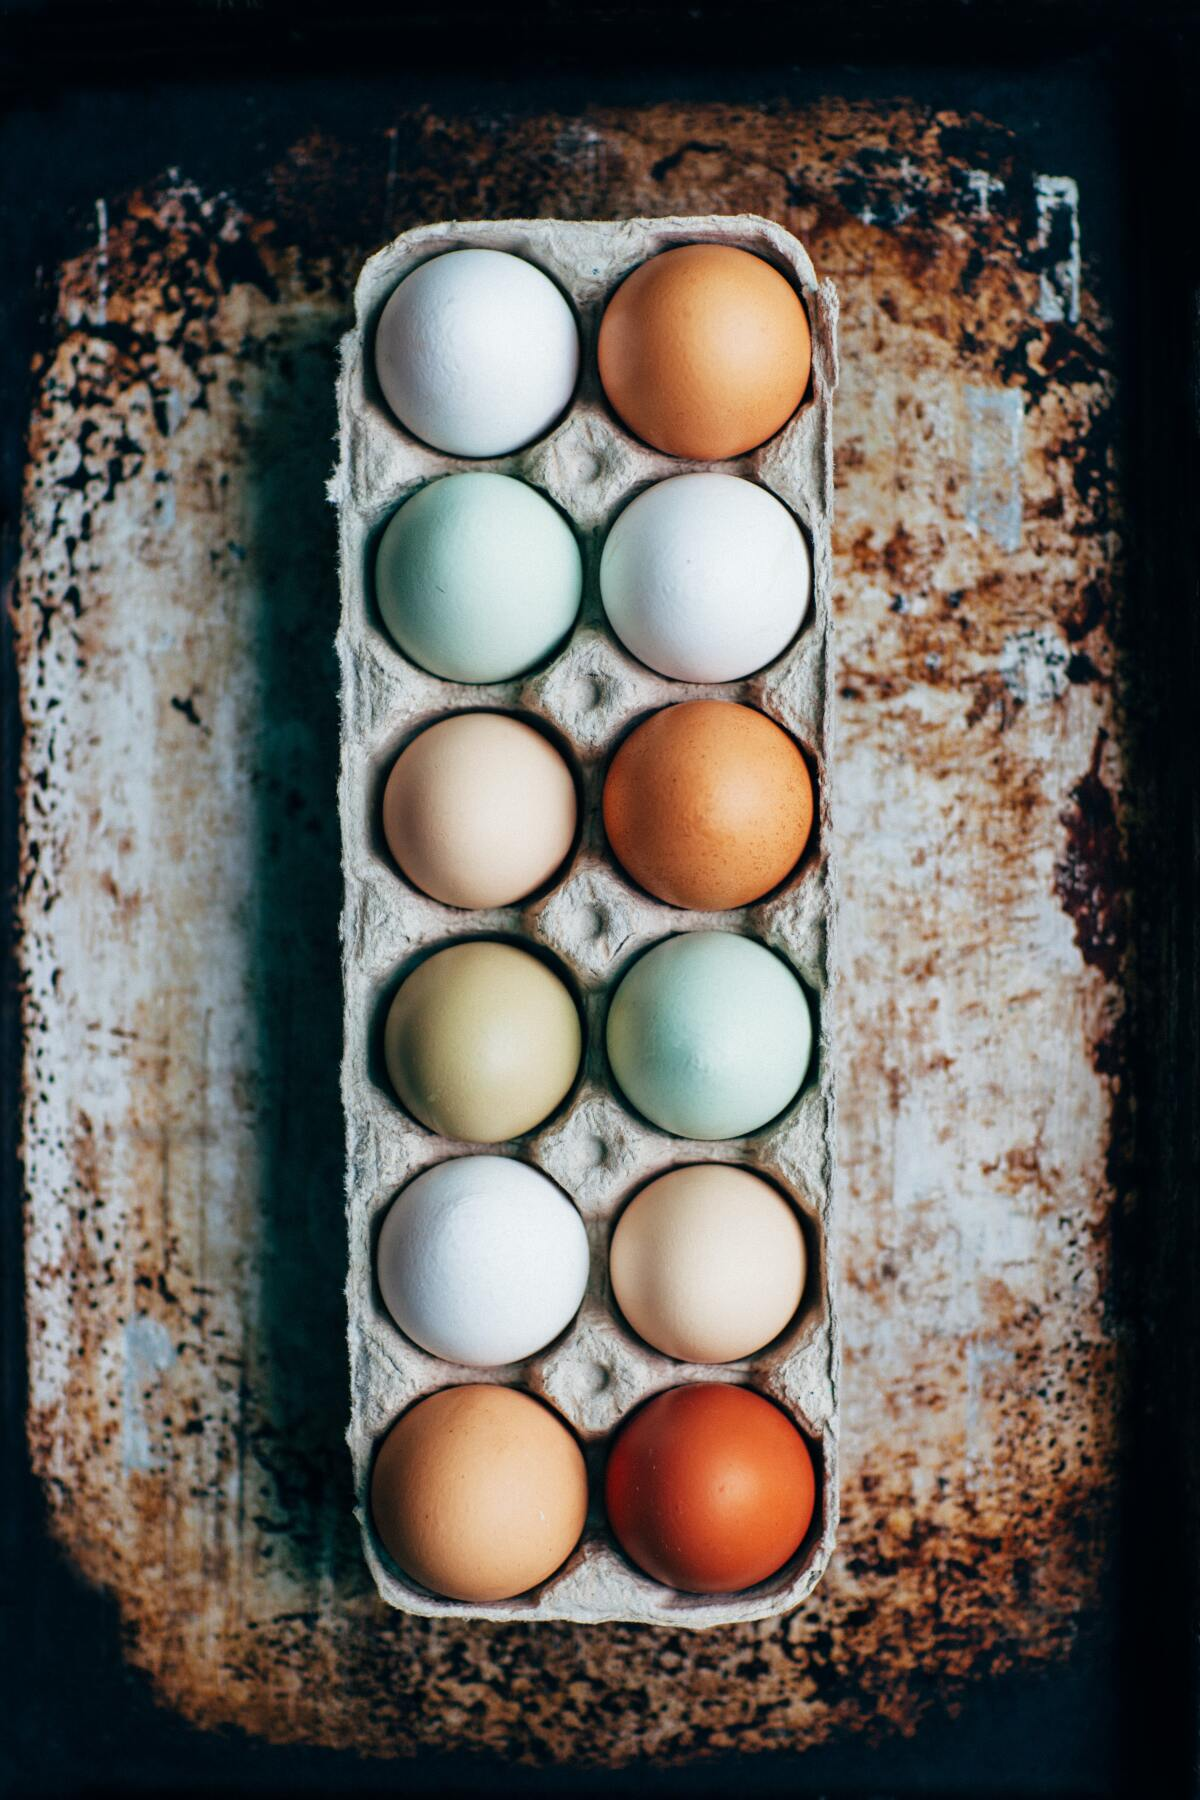
\includegraphics[width=.9\textwidth]{eggs.jpg}}
  \end{minipage}
\end{frame}

\begin{frame}
  \frametitle{OTRAS COSAS QUE SE VENDEN POR DOCENA}

  \begin{center}
    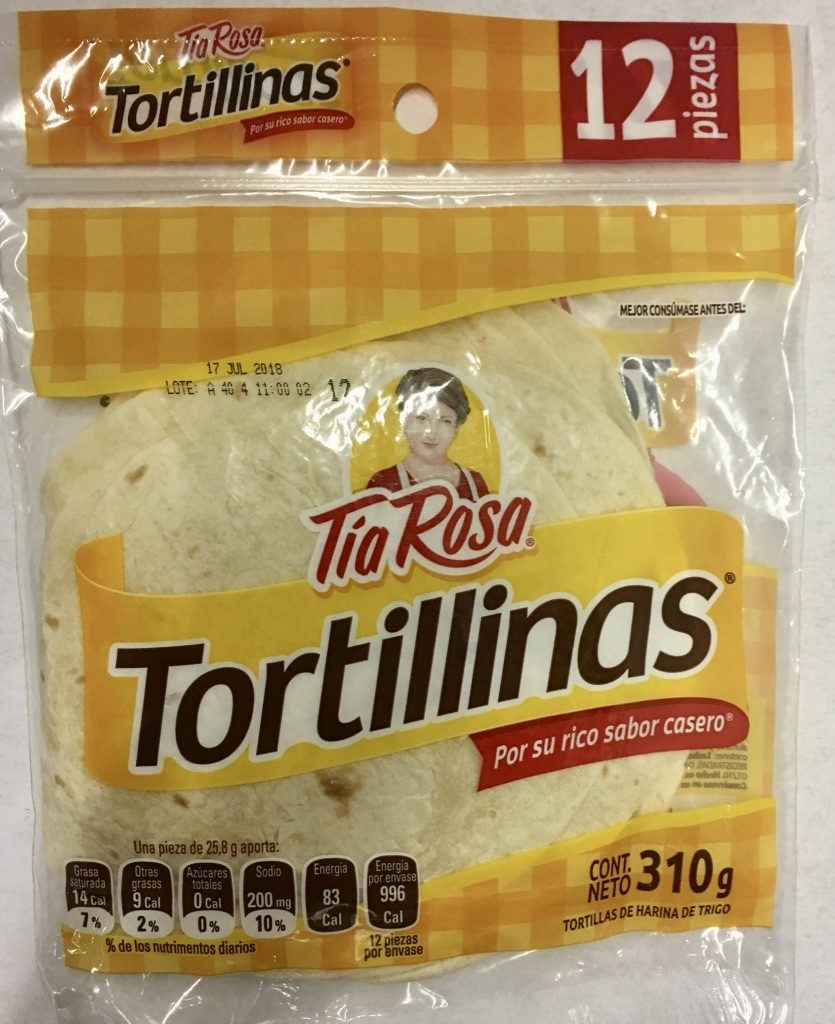
\includegraphics[width=0.4\textwidth]{tia-rosa.jpg}
  \end{center}
\end{frame}

\begin{frame}
  \frametitle{EJEMPLO: 60 MINUTOS Y 60 SEGUNDOS}

  \begin{minipage}[t][0.6\textheight]{0.6\textwidth}
    \vspace{0pt}
    \begin{itemize}
    \item<2-> Los divisores (positivos) de $60$ son
      $1$, $2$, $3$, $4$, $5$, $6$, $10$, $12$, $15$, $20$, $30$, $60$.

    \item<3-> Muy cómodo dividir una hora en $60$ minutos y un minuto en $60$
      segundos.

    \item<4-> $100$ tiene menos divisores:

      $1$, $2$, $4$, $5$, $10$, $20$, $25$, $50$, $100$.

    \item<5-> Influencia muy antigua babilónica (c. 2000 a.C.):

      sistema de numeración \textbf{sexagesimal} (base $60$).
    \end{itemize}
  \end{minipage}
  \begin{minipage}[t]{0.35\textwidth}
    \vspace{0pt}\flushright
    \onslide<2->{
\includegraphics[width=.9\textwidth]{clock.jpg}}
  \end{minipage}
\end{frame}

\begin{frame}
  \frametitle{NUMERACIÓN BABILÓNICA}

  \begin{center}
    
\includegraphics[width=\textwidth]{babylonian.pdf}
  \end{center}
\end{frame}

\begin{frame}
  \frametitle{EJEMPLO: 360 GRADOS}

  \begin{minipage}[t][0.8\textheight]{0.6\textwidth}
    \vspace{0pt}
    \begin{itemize}
    \item<2-> La división del círculo en $360$ \textbf{grados} viene de la misma
      influencia babilónica.

    \item<3-> $360 = 6 \cdot 60$.

    \item<4-> Divisores (positivos) de $360$:

      $1$, $2$, $3$, $4$, $5$, $6$, $8$, $9$, $10$, $12$, $15$, $18$, $20$,
      $24$, $30$, $36$, $40$, $45$, $60$, $72$, $90$, $120$, $180$, $360$.

    \item<5-> Convención totalmente arbitraria, pero práctica.

    \item<6-> Los matemáticos de hoy dividen el círculo en 2π \textbf{radianes}.
    \end{itemize}
  \end{minipage}
  \begin{minipage}[t]{0.35\textwidth}
    \vspace{0pt}\flushright
    \onslide<2->{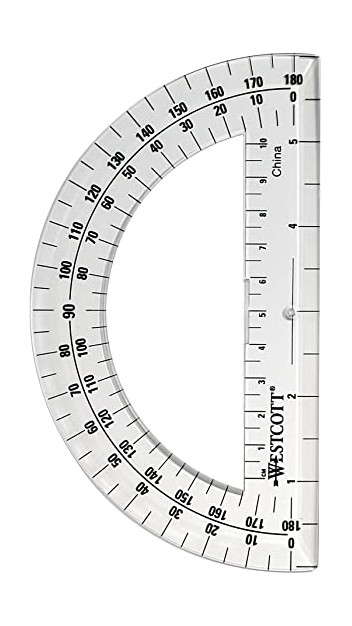
\includegraphics[width=.9\textwidth]{protractor.jpg}}
  \end{minipage}
\end{frame}

\begin{frame}
  \frametitle{EJEMPLO: COORDENADAS GEOGRÁFICAS}

  \begin{minipage}[t][0.8\textheight]{0.6\textwidth}
    \vspace{0pt}
    \begin{itemize}
    \item<2-> Hiparco de Nicea \\
      (c. 190 a.C. -- 120 a.C.):

      la división del día en $24$ horas,

      las \textbf{coordenadas geográficas}.

    \item<3-> Influencia babilónica.

    \item<4-> Latitud $0$--$180^\circ$ norte / sur.

    \item<5-> Longitud $0$--$180^\circ$ este / oeste.

    \item<6-> $60$ minutos (${}'$) en cada grado.

    \item<7-> $60$ segundos (${}''$) en cada minuto.

    \item<8-> Ejemplo: la Ciudad de México,

      $19^\circ$ $25'$ $10''$ N,
      $99^\circ$ $8'$ $44''$ O.
    \end{itemize}
  \end{minipage}
  \begin{minipage}[t]{0.35\textwidth}
    \vspace{0pt}\flushright
    \onslide<2->{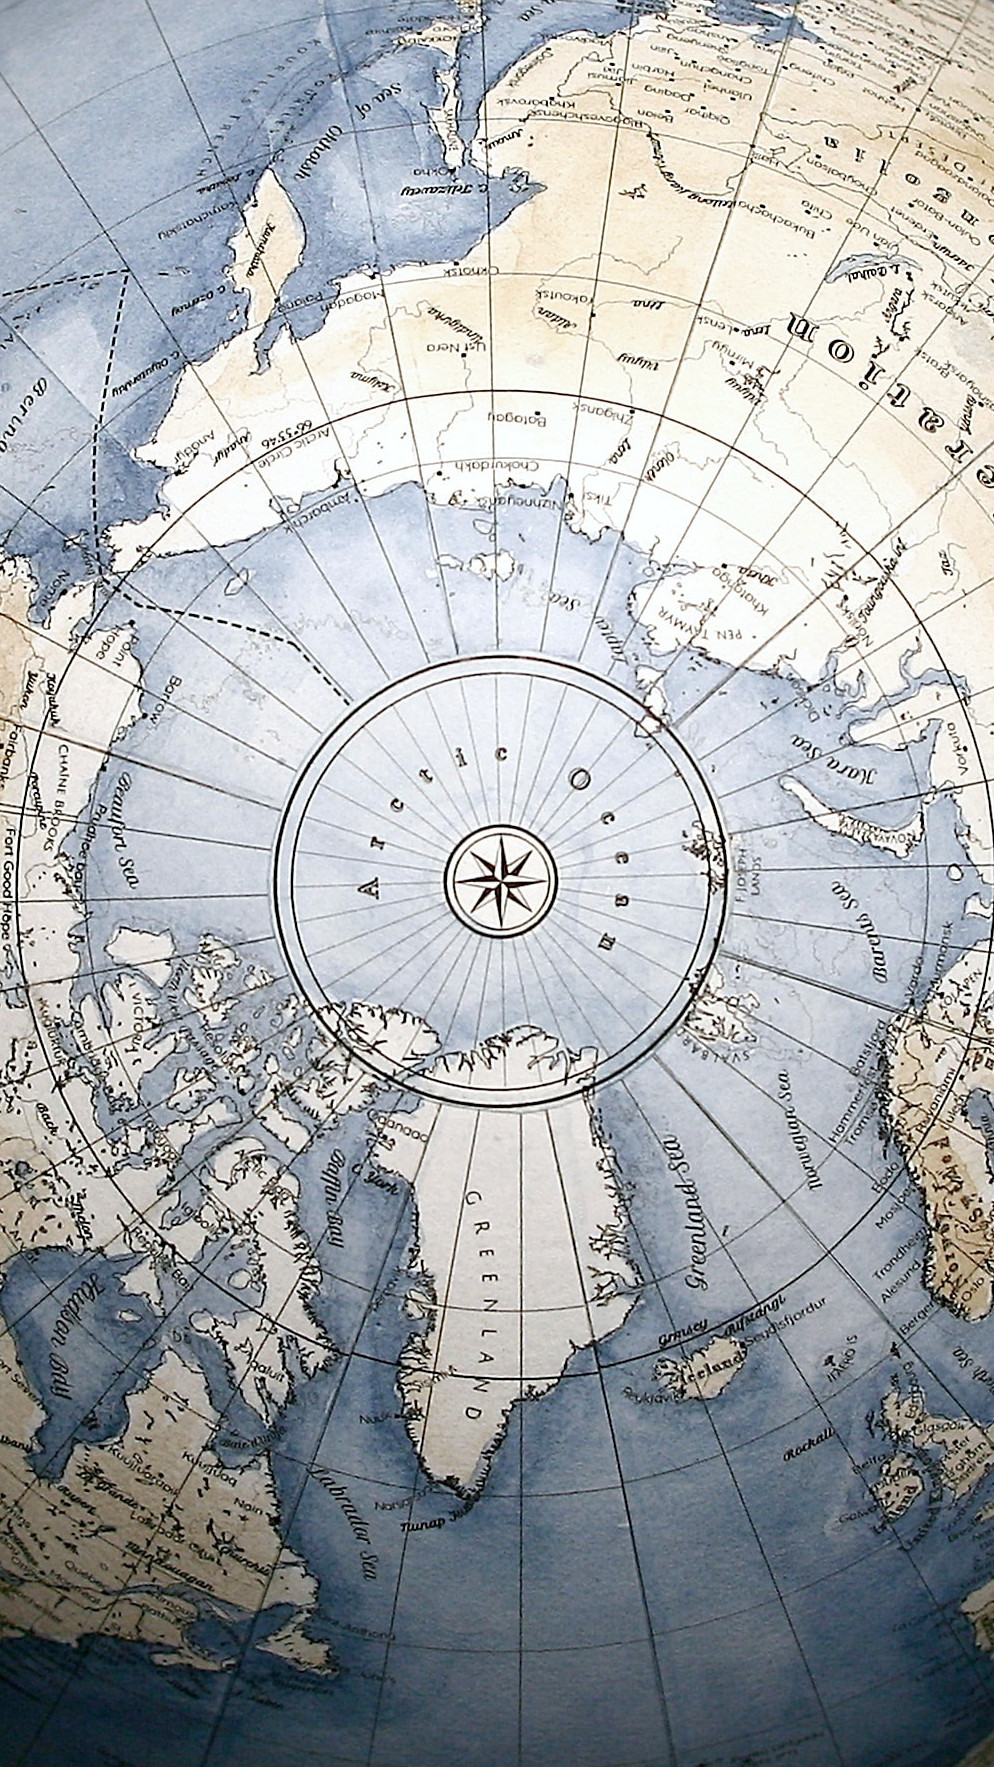
\includegraphics[width=.9\textwidth]{globe.jpg}}
  \end{minipage}
\end{frame}

\begin{frame}
  \frametitle{NÚMEROS PRIMOS}

  \begin{itemize}
  \item<2-> $7$ tiene como sus divisores $\pm 1$ y $\pm 7$.

  \item<3-> $23$ tiene como sus divisores $\pm 1$ y $\pm 23$.

  \item<4-> Son \textbf{números primos}.

  \item<5-> $360$ tiene muchos divisores, pero

    $359$ es divisible solo por $\pm 1$ y $\pm 359$; es primo.

  \item<6-> Los primeros primos son

    $2$, $3$, $5$, $7$, $11$, $13$, $17$, $19$, $23$, $29$, $31$, $37$, $41$,
    $43$, $47$, $53$, $59$, $61$, $67$, $71$, $73$, $79$, $83$, $89$, $97$,
    $101$, $\ldots$

  \item<7-> El número $\pm 1$ no se considera como primo.
  \end{itemize}
\end{frame}

\begin{frame}
  \frametitle{PROPIEDADES DE DIVISIBILIDAD}

  \begin{itemize}
  \item<2-> Si $b \mid a$, entonces $|b| \le |a|$.

    \onslide<3->{\emph{Demostración}: si $a = bc$, entonces $|a| = |b|\cdot |c|$.}

  \item<4-> \textbf{Corolario}: si $b \mid a$ y $a \mid b$, entonces
    $a = \pm b$.

    \onslide<5->{(Relación \textbf{antisimétrica}, salvo signo.)}
  \end{itemize}
\end{frame}

\begin{frame}
  \frametitle{PROPIEDADES DE DIVISIBILIDAD (CONT.)}

  \begin{enumerate}
  \item<2->[1)] $1\mid a$, $a \mid a$, $a \mid 0$ para cualquier $a$,

  \item<3->[2)] $a\mid 1$ si y solamente si $a = \pm 1$,

  \item<4->[3)] $0\mid a$ si y solamente si $a = 0$,

  \item<5->[4)] si $c \mid a$ y $c \mid b$, entonces $c \mid (a \pm b)$,

  \item<6->[5)] \textbf{transitividad}:

    si $c \mid b$ y $b \mid a$, entonces $c \mid a$,

  \item<7->[6)] \textbf{cancelación}:

    si $c \ne 0$, entonces
    $ac \mid bc$ implica $a\mid b$,

  \item<8->[7)] $b \mid a$ si y solamente si $-b \mid a$.
  \end{enumerate}

  \onslide<9->{\emph{Demostración}. Ejercicio (!)}
\end{frame}

\begin{frame}
  \frametitle{ORDEN PARCIAL SOBRE LOS NATURALES}

  \[ \begin{tikzpicture}[font=\small,x=1.75em, y=1.5em, every node/.style={inner sep=2pt,outer sep=0pt}]
      \draw (0,0) node (n1) {$1$};
      \draw (-1,2) node[circle, draw=white] (n2) {$2$};
      \draw (0,3) node[circle, draw=white] (n3) {$3$};
      \draw (-2,4) node (n4) {$4$};
      \draw (+2,5) node[circle, draw=white] (n5) {$5$};
      \draw (-1,6) node (n6) {$6$};
      \draw (+6,7) node[circle, draw=white] (n7) {$7$};
      \draw (-4,8) node (n8) {$8$};
      \draw (+2,9) node (n9) {$9$};
      \draw (0,10) node (n10) {$10$};
      \draw (+7,11) node[circle, draw=white] (n11) {$11$};
      \draw (-2,12) node (n12) {$12$};

      \draw (n1) -- (n2);
      \draw (n1) -- (n3);
      \draw (n1) -- (n5);
      \draw (n1) -- (n7);
      \draw (n1) -- (n11);

      \draw (n2) -- (n4);
      \draw (n2) -- (n6);
      \draw (n2) -- (n10);

      \draw (n3) -- (n6);
      \draw (n3) -- (n9);

      \draw (n4) -- (n8);
      \draw (n4) -- (n12);

      \draw (n5) -- (n10);

      \draw (n6) -- (n12);

      \draw (n1) -- ($(n1)+(-0.25,1)$);
      \draw (n2) -- ($(n2)+(0,1)$);
      \draw (n3) -- ($(n3)+(0,1)$);
      \draw (n4) -- ($(n4)+(-0.25,1)$);
      \draw (n5) -- ($(n5)+(0,1)$);
      \draw (n6) -- ($(n6)+(0,1)$);
      \draw (n7) -- ($(n7)+(0,1)$);
      \draw (n8) -- ($(n8)+(0,1)$);
      \draw (n9) -- ($(n9)+(0,1)$);
      \draw (n10) -- ($(n10)+(0,1)$);
      \draw (n11) -- ($(n11)+(0,1.5)$);
      \draw (n12) -- ($(n12)+(0,1)$);
    \end{tikzpicture} \]
  \end{frame}

  \begin{frame}
    \frametitle{A CONTINUACIÓN}

    \begin{itemize}
    \item<2-> \textbf{División con residuo} (= \textbf{división euclidiana}).

    \item<3-> Ejemplo: $3\nmid 20$, pero

      \[ \frac{20}{3} = 6\,\frac{2}{3}
        \iff
        20 = 6\cdot 3 + 2. \]

      $2$ es el \textbf{residuo} de división.

    \item<4-> \textbf{Numeración en la base $b$}.

    \item<5-> Ejemplo: $20 = 2^4 + 2^2$, así que

      $20 = \text{\texttt{10100}}$ en la base $2$.
    \end{itemize}
  \end{frame}

\begin{frame}[plain,noframenumbering]

  \vfill

  \begin{center}\huge\headingfont
    ¡GRACIAS POR SU ATENCIÓN!
  \end{center}

  \vfill
\end{frame}
\end{document}
